% status: 2
% chapter: Security

\title{Financial Analysis Service}

\author{Rashmi Ray}
\affiliation{%
  \institution{Indiana University}
  \streetaddress{107 S. Indiana Avenue}
  \city{Bloomington}
  \state{Indiana}
  \postcode{43017-6221}
}
\email{rashray@iu.edu}
% The default list of authors is too long for headers}

\renewcommand{\shortauthors}{Rashmi Ray}

\begin{abstract}
The project involves creating a Kubernete cluster in GoogleCloud and later 
automating the installation and setup process by including the shell script.
The same process will be executed in a Kubernetes Chameleon cluster. The shell
script will be modified as needed. The project will also involve developing a 
stock API using flask that will provide real-time analysis of the stock market 
data. The performance of the API will be compared in both Chameleon and 
GoogleCloud. The stock API will be using python, pyGal, Quandl. The 
benchmarking process will be registered in the project report. 

The main idea behind the project was to compare and contrast ease of 
Kubernetes deployment in 

\end{abstract}

\keywords{hid-sp18-417, Kubernetes, deloyment, performance, GKE, containers}


\maketitle

\section{Introduction}

The area of research for this project is Kubernetes. Looking at the
high popularity of the tool, it is becoming a buzz word in the world
of cloud computing and containers. The project compares and contrasts
the ease of deployment, configuration and performance in different
systems. Before going into the detail of the project outcome, it is
important to introduce several key components of the project.

\section{Kubernetes}

Kubernetes is an open-source system developed and maintained by Google
Inc.  The system provides a container orchestration platform for ease
of deployment, management and scaling of services and resources. The
system places containers automatically based on it resource
requirement not compromising availability.  Similarly, it provides
seamless management of data volumes and storage system.  It allows
updating configurations of the deployment without rebuilding the
image. The system can facilitate public, private or hybrid container
management system based on an organization's requirement.  Kubernetes
resource monitoring system oversees automatic rollout and rollback of
the resources in case of fallbacks.


Kubernetes is also known as K8 or kube. This is originally developed
based on Google's container management system. A Kubernetes can be
deployed in a single host, but it is designed to be benefitted
efficiently when used for a cluster of connected hosts. Use of a
cluster of multiple hosts facilitates high availability.


The primary components of the system are: 

The master node controls the other nodes. Nodes are the hosts in the
cluster.  Pod is a group of one or more containers deployed in a node.
The Replication Controller monitors and controls the replicas of the
services. A Kubernetes service is a single unit that has a collection
of rules/configuration for effective deployment of a
container. Various metadata such as replicas, environment, track,
port, can be defined in a service configuration.  Kubectl is the
command line configuration tool provided by Kubernetes.

The figure Figure~\ref{fig:kube-archtecture} below explains the
Kubernetes architecture. The master is responsible for managing the
deployments, scheduling, exposing containerized applications.

\begin{figure}[htb]
	\centering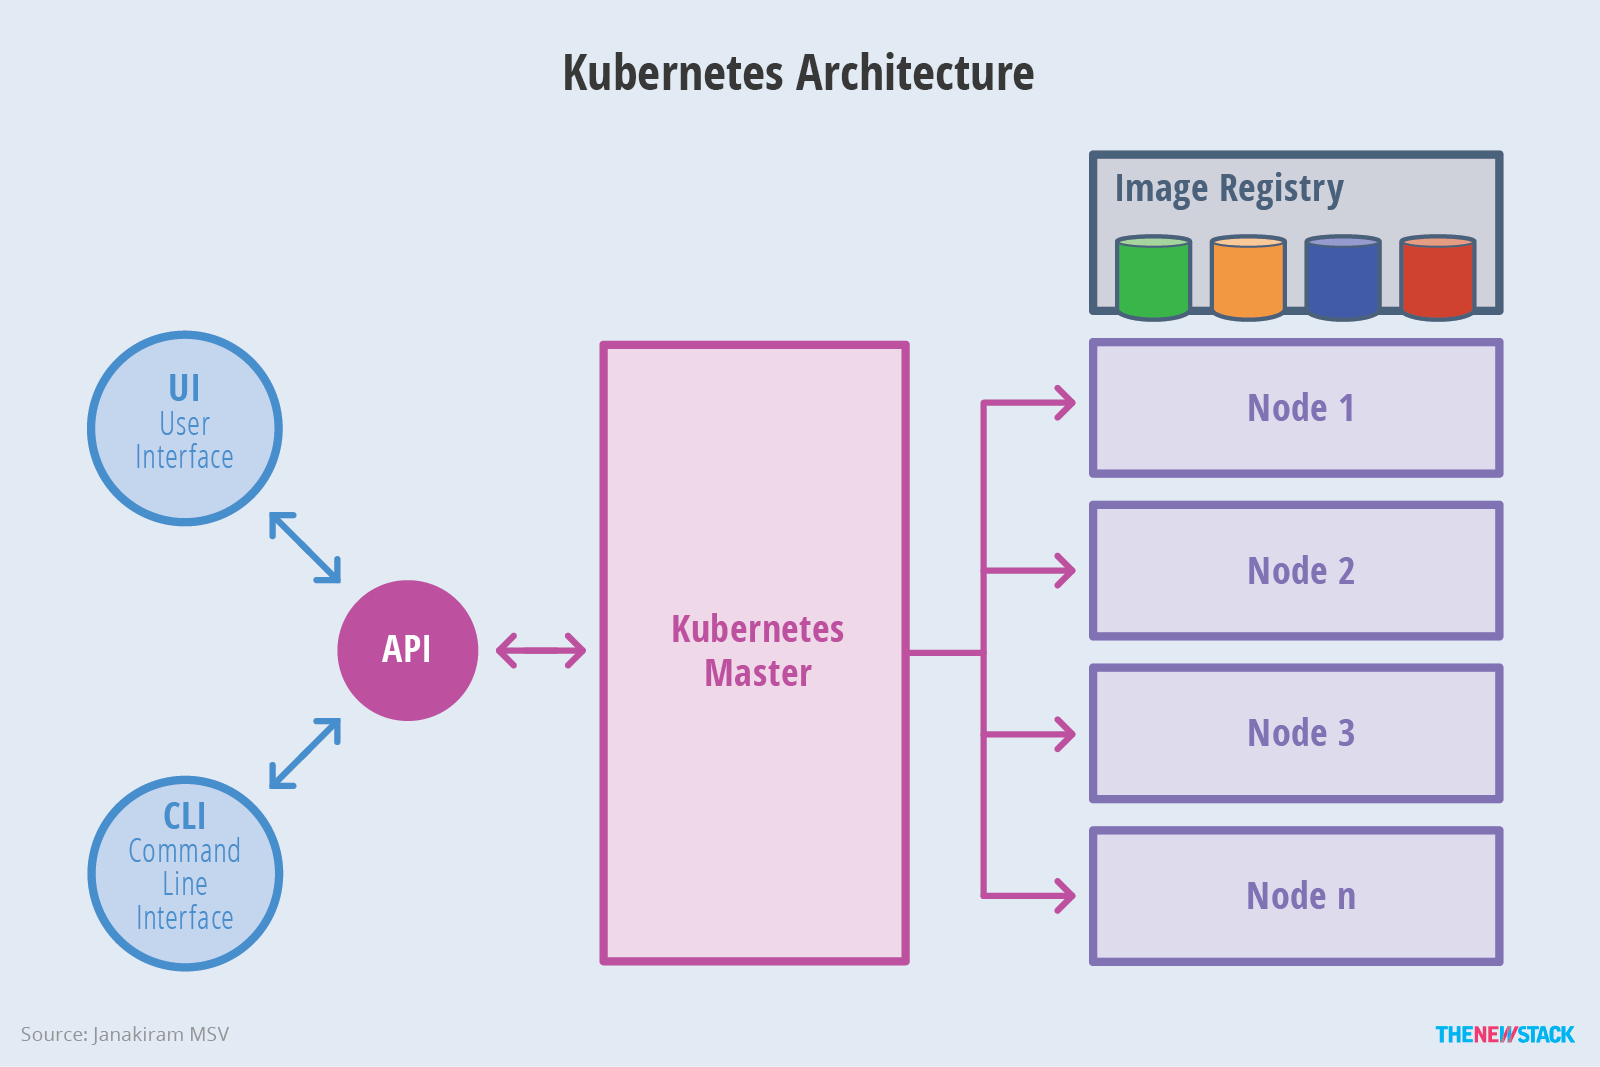
\includegraphics[width=\columnwidth]{images/hid_417_Kubernetes-Architecture.png}
  \caption{Kubernetes Architecture~\cite{hid-sp18-417-kubernetes}}
  \label{fig:kube-archtecture}
\end{figure}

\section{ Google Kubernetes Engine GKE}

Google Kubernetes Engine is the tool developed by Google Inc to
simplify the management and orchestration of Kubernetes systems, in
Google's public cloud services. This will help an organization focus
more into their ow product development than worrying about Kubernetes
networking, upgrades and maintenance. As the main focus of the project
was Kubernetes, it was vital for the author to include GKE in the
scope of the project.

\subsection{benefits}

Here are some benefits: With use of GKE, user need not worry about
Kubernetes master. The system ensures that master is always up and
running. User need not worry about underlying networking on what to
user e.g. weave, flannel etc.  It makes access and identity management
easier with Google's Identity and Container Management System
\TODO{[IAM]}. Auto scaling is easier with just simple commands. With
Kubernetes' frequent releases it is important for the system to stay
updated always. The upgrade is easier with gcloud with just a single
command rather than the manual overhead of porting the system step by
step.

\subsection{Initial Setup}

The project availed the free tier offer from Google to bring in the
setup and configuration experience for GKE. As of Apr 2018, Google is
offering a 300 dollar credit to be used with in 12 months. The free
trial has certain resource usage limitations applied. Please refer to
Google's documentation for details.  But the bottom-line was that the
limitation was well within the projects scope to explore the cluster's
performance so the author decided to go ahead with the research.

Here are the key steps involved to get you started with GKE:

\begin{description}

\item[Account Setup] Before you can use GKE, you need to register to
  google cloud. You can use an existing google account. It is required
  to provide credit card information.  Google assures that the card
  won't be charged without your permission.

https://cloud.google.com/signin

\item[Shell Setup] GKE provides an option of using google cloud shell
  [from the browser - no installation needed] or local shell [gcloud
  installation]. The project kept the local setup in the scope. So
  here is the command set to create environment variable, import
  public key, and install Google SDK.

\begin{verbatim}
# Create environment variable for correct distribution
 export CLOUD_SDK_REPO='cloud-sdk-$(lsb_release -c -s)'

# Add the Cloud SDK distribution URI as a package source
echo 'deb http://packages.cloud.google.com/apt $CLOUD_SDK_REPO main' | 
sudo tee -a /etc/apt/sources.list.d/google-cloud-sdk.list

# Import the Google Cloud Platform public key
curl https://packages.cloud.google.com/apt/doc/apt-key.gpg | sudo apt-key add -

# Update the package list and install the Cloud SDK
sudo apt-get update && sudo apt-get install google-cloud-sdk
\end{verbatim}

\item[Install Kubernetes] Now install Kubernetes:

\begin{verbatim}
sudo apt-get install kubectl
\end{verbatim}

\item[Initiate GoogleCloud] Now GKE is ready to be initiated locally. Before 
initiating it is 
important to know that you will setup the project and compute zone during the 
setup. You can setup the compute zone later but it is advised to set your 
preference at the beginning to ensure that your requests are directed in the 
nearest processing center. [Still to discover more about zones, but went ahead 
a selected central-zone-1] 

Now ready to initiate gcloud:
\begin{verbatim}
  gcloud init
\end{verbatim}

\item[Create Cluster] A cluster consists of one master multiple worker 
machines.  gcloud creates a cluster of three nodes by default. This takes
 couple of  seconds. Once done it is important to get the credential, so that
  containers can be deployed gcloud container clusters create
  [\verb|CLUSTER_NAME|] in
   the cluster
  \begin{verbatim}
    gcloud container clusters create [CLUSTER_NAME]
  \end{verbatim}
\item[Deployment] A containerized docker image can be deployed to the cluster 
using the following:
\begin{verbatim}
  kubectl run [SERVICE_NAME] --image [IMAGE_NAME] --port [port number]
\end{verbatim}
\item [Exposing Service] Exposing a service to a port will enable external 
access:
[A loadbalancer exposes the service externally.]
\begin{verbatim}
  kubectl expose deployment [SERVICE_NAME] --type 'LoadBalancer'
\end{verbatim}

Once exposed it may take a moment for the service to get exposed. The
external IP can be fetched using the following:

\begin{verbatim}
  kubectl get service [SERVICE_NAME]
\end{verbatim}

\item [External Access] Once the IP is shown, the exposed contained can be 
accessed in any web browser.
\begin{verbatim}
  http://[EXTERNAL_IP]:[EXPORTED_PORT]
\end{verbatim}

\item [Cleanup] Finally, here are some useful clean up commands:
\begin{verbatim}
  kubectl delete pod [POD_NAME]
  kubectl delete service [SEVICE_NAME]
  kubectl delete deployment [DEPLOYMENT_NAME]
  gcloud container clusters delete [CLUSTER_NAME]
\end{verbatim}

  Please keep in mind that if a pod is generated through a deployment
  then to remove it the deployment has to be deleted. Deleting the pod
  will regenerate the pod because the replication manager is
  monitoring the failure and handling them.

\end{description}

This Figure~\ref{fig:gcloud-dashboard} shows the GKE dashboard in the current 
state. Where the current 
balance is shown in the top-left corner. In the left menu option will provide 
the current state of the account. The first dox in the main content area is 
showing the current project in use. Currently it is a new project with no
 clusters so there is not much to report.
 
 \begin{figure}[htb]
   \centering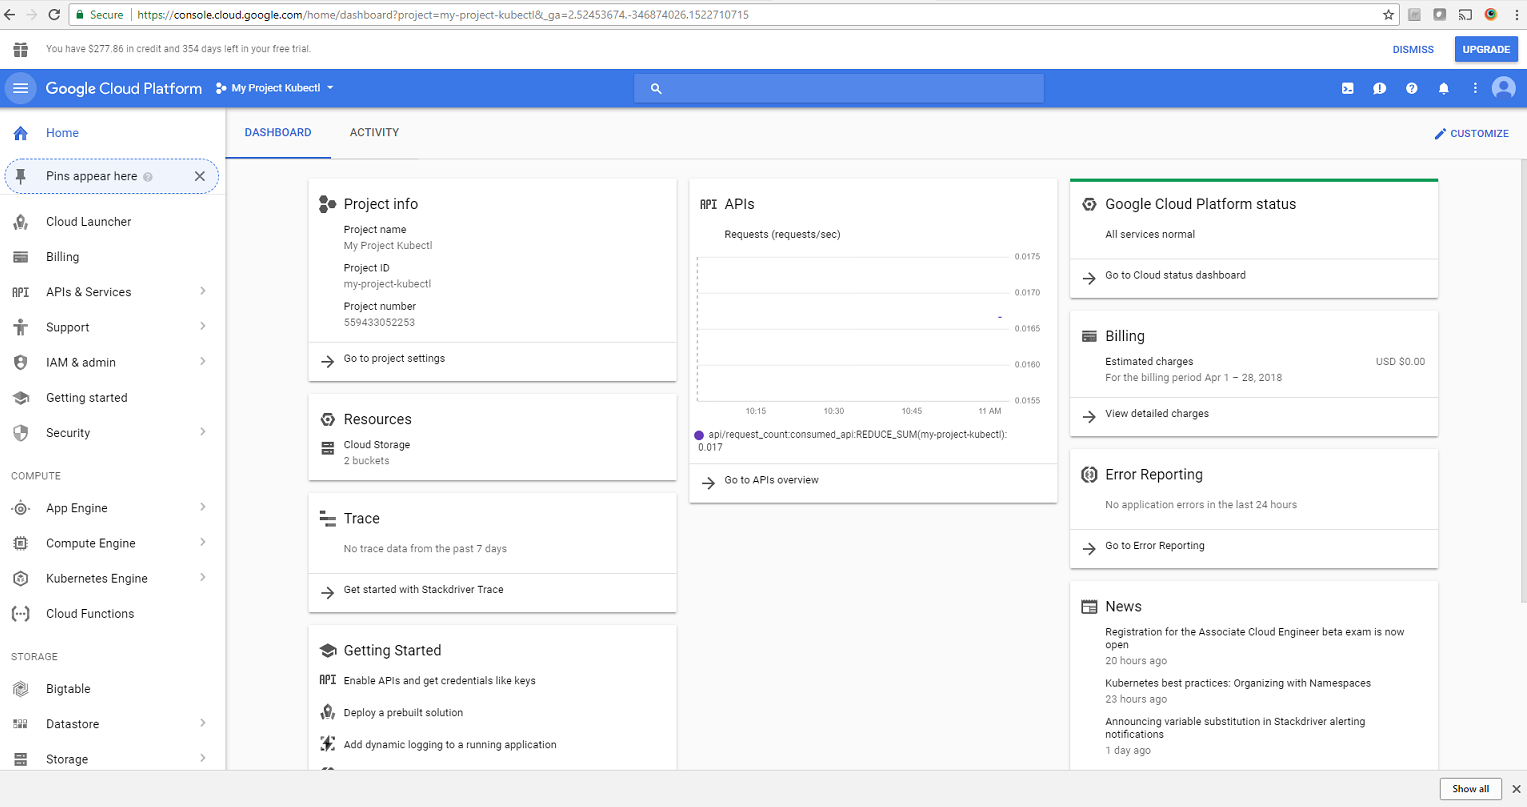
\includegraphics[width=\columnwidth]{images/hid_417_gcloud_browser.png}
   \caption{gcloud Dashboard}\label{fig:gcloud-dashboard}
 \end{figure}

 \section{API in Use}

\TODO{paragraph missing}

\subsection{Python API}

\TODO{Python API control structure and available features are discussed}

\subsection{Flask Service}

\TODO{the details of the swagger service in use}

\subsection{setup process}

\TODO{Initial setup experience is discussed}

\subsection{Chameleon}

\TODO{JetStream setup is discussed.}

\subsection{Stocks Analysis}

\TODO{Practice use of the webservice and the current 
market trend of tools and technologies in the context is discussed.}

\subsection{Trouble shooting}

\TODO{Troubleshooting experience during the project is logged}

\section{BenchMarking}

\TODO{Compare and contrast the installation, setup and performance of the 
service in Pi and Jetstream cluster}


\section{Conclusion}

\TODO{Put here an conclusion.} Conclusion and abstracts must not have any
citations in the section.


\begin{acks}
The author would like to thank Dr.\ Gregor von Laszewski for his support and 
suggestions in writing this paper.
\end{acks}

\bibliographystyle{ACM-Reference-Format}
\bibliography{report}



